\section{W5: Agile Estimations and Planning}

\textbf{Understand Agile SDLC Planning and Estimation Techniques.}

\textbf{Requirement gathering in Traditional and Agile.}
    \textbf{User Stories}: characteristics follow INVEST (Independent, Negotiable, Valuable, Estimable, Small, Testable).

    \textbf{Epics}: large user stories that cannot be completed in a single iteration.

    \textbf{Acceptance Criteria (AC's)}: conditions that a software product must satisfy to be accepted by a user, customer, or other stakeholders.

    \textbf{Definition of Done (DoD)}: a shared understanding of what it means for work to be complete.



\textbf{Scrum Artefacts.}

\textbf{Agile Estimations.}

    \textbf{Velocity}: measure of the amount of work a team can tackle during a single sprint. V = \# of team members * SP per day * \# of days in sprint.

\textbf{Agile Planning.}

    \textbf{MoSCoW}: Must have, Should have, Could have, Won't have.

    \textbf{Planning Artefacts}
    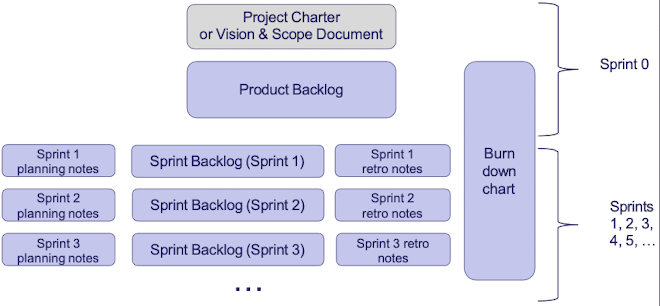
\includegraphics[width=\linewidth]{figs/SCR-20240606-lcfi.png}
